\documentclass[tikz,border=3pt]{standalone}
\usepackage{amsmath,amssymb,bm}
\usetikzlibrary{arrows.meta,calc,fit,backgrounds,decorations.pathreplacing}
\definecolor{dblue}{HTML}{08519C}
\definecolor{mblue}{HTML}{9ECAE1}
\definecolor{lblue}{HTML}{EAF2FA}
\newcommand{\ket}[1]{|#1\rangle}
\begin{document}
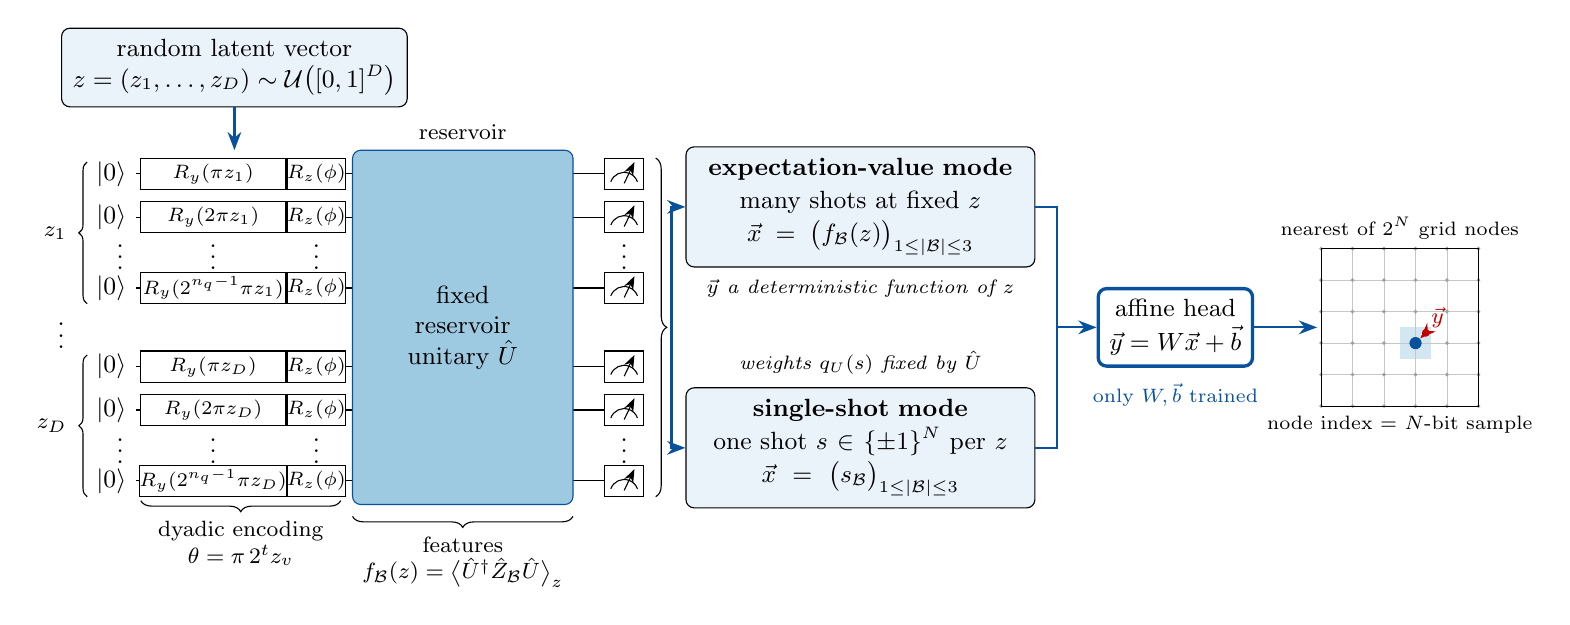
\begin{tikzpicture}[>=Stealth,font=\small,
  gate/.style={draw,fill=white,minimum width=0.66cm,minimum height=0.40cm,inner sep=0pt,font=\scriptsize},
  cliff/.style={draw=dblue,fill=mblue,rounded corners=1pt},
  box/.style={draw,rounded corners=3pt,fill=lblue,align=center,inner sep=4pt},
  arr/.style={->,thick,dblue}]

\def\yA{0}\def\yB{-0.55}\def\yC{-1.45}\def\yD{-2.45}\def\yE{-3.0}\def\yF{-3.9}
\foreach \y/\ang in {\yA/\pi z_1,\yB/2\pi z_1,\yC/2^{n_q-1}\pi z_1,\yD/\pi z_D,\yE/2\pi z_D,\yF/2^{n_q-1}\pi z_D}{
  \node[left] at (0,\y) {$\ket0$};
  \draw (0,\y) -- (2.75,\y);
  \draw (5.55,\y) -- (5.95,\y);
  \node[gate,minimum width=1.85cm] at (0.98,\y) {$R_y(\ang)$};
  \node[gate] at (2.29,\y) {$R_z(\phi)$};
  \draw[fill=white] (5.95,\y-0.2) rectangle (6.45,\y+0.2);
  \draw (6.03,\y-0.1) arc (160:20:0.18);
  \draw[->,>=Stealth] (6.2,\y-0.12) -- (6.33,\y+0.15);
}
\foreach \y in {-0.95,-3.42}{
  \node at (-0.2,\y) {$\vdots$}; \node at (0.98,\y) {$\vdots$}; \node at (2.29,\y) {$\vdots$}; \node at (6.2,\y) {$\vdots$};
}
\node at (-0.95,-1.95) {$\vdots$};
\draw[decorate,decoration={brace,amplitude=3pt}] (-0.62,-1.65) -- (-0.62,0.15) node[midway,left=4pt,font=\footnotesize] {$z_1$};
\draw[decorate,decoration={brace,amplitude=3pt}] (-0.62,-4.1) -- (-0.62,-2.3) node[midway,left=4pt,font=\footnotesize] {$z_D$};
\node[box,align=center] (z) at (1.25,1.35) {random latent vector\\ $z=(z_1,\dots,z_D)\sim\mathcal U\big([0,1]^D\big)$};
\draw[arr] (z.south) -- (1.25,0.3);
\draw[decorate,decoration={brace,mirror,amplitude=4pt}] (0.06,-4.15) -- (2.6,-4.15)
  node[midway,below=4pt,align=center,font=\footnotesize] {dyadic encoding\\ $\theta=\pi\,2^{t}z_v$};

\node[draw=dblue,fill=mblue,rounded corners=3pt,minimum width=2.8cm,minimum height=4.5cm,align=center] (U) at (4.15,-1.95) {fixed\\ reservoir\\ unitary $\hat U$};
\node[above,align=center,font=\footnotesize] at (U.north) {reservoir};
\draw[decorate,decoration={brace,mirror,amplitude=4pt}] (2.75,-4.35) -- (5.55,-4.35)
  node[midway,below=4pt,align=center,font=\footnotesize] {features\\ $f_{\mathcal B}(z)=\big\langle\hat U^\dagger\hat Z_{\mathcal B}\hat U\big\rangle_z$};

\draw[decorate,decoration={brace,amplitude=4pt}] (6.6,0.2) -- (6.6,-4.1);
\coordinate (m) at (6.8,-1.95);

\node[box,text width=4.15cm] (E) at (9.2,-0.42) {%
  \textbf{expectation-value mode}\\[1pt]
  many shots at fixed $z$\\[1pt]
  $\vec x=\big(f_{\mathcal B}(z)\big)_{1\le|\mathcal B|\le3}$};
\node[box,text width=4.15cm] (S) at (9.2,-3.48) {%
  \textbf{single-shot mode}\\[1pt]
  one shot $s\in\{\pm1\}^N$ per $z$\\[1pt]
  $\vec x=\big(s_{\mathcal B}\big)_{1\le|\mathcal B|\le3}$};
\draw[arr] (m) |- (E.west);
\draw[arr] (m) |- (S.west);
\node[font=\scriptsize\itshape,align=center,below=1pt] at (E.south) {$\vec y$ a deterministic function of $z$};
\node[font=\scriptsize\itshape,align=center,above=1pt] at (S.north) {weights $q_U(s)$ fixed by $\hat U$};

\node[box,draw=dblue,very thick,fill=white] (H) at (13.2,-1.95) {affine head\\[1pt] $\vec y=W\vec x+\vec b$};
\node[font=\scriptsize,dblue,below=2pt] at (H.south) {only $W,\vec b$ trained};
\draw[thick,dblue] (E.east) -| (11.7,-1.95);
\draw[thick,dblue] (S.east) -| (11.7,-1.95);
\draw[arr] (11.7,-1.95) -- (H.west);

\begin{scope}[shift={(15.05,-2.95)}]
  \fill[mblue!45] (1.0,0.6) rectangle (1.4,1.0);
  \draw[step=0.4,gray!45,very thin] (0,0) grid (2.0,2.0);
  \foreach \a in {0,0.4,...,2.01}{\foreach \b in {0,0.4,...,2.01}{\fill[gray!75] (\a,\b) circle (0.7pt);}}
  \draw (0,0) rectangle (2.0,2.0);
  \draw[->,>=Stealth,red!75!black,semithick,shorten >=2.4pt] (1.33,0.93) -- (1.2,0.8);
  \fill[dblue] (1.2,0.8) circle (2.2pt);
  \fill[red!75!black] (1.33,0.93) circle (1.4pt);
  \node[red!75!black,font=\footnotesize,anchor=south west,inner sep=1pt] at (1.36,0.95) {$\vec y$};
  \node[font=\scriptsize,above,align=center] at (1.0,2.0) {nearest of $2^N$ grid nodes};
  \node[font=\scriptsize,below,align=center] at (1.0,0) {node index $=$ $N$-bit sample};
\end{scope}
\draw[arr] (H.east) -- (15.0,-1.95);
\end{tikzpicture}
\end{document}
